% Hand-written narrative; every number is a macro from generated/numbers.tex.
\textbf{Precision.} At 10 alerts per day BudgetAwareConformal reaches $\text{P@10}=\POursBA$,
against \PIFBA{} for Isolation Forest, \PLOFBA{} for LOF,
\PAEBA{} for the autoencoder and \PRulesBA{} for the signature rules. The relative gain over
Isolation Forest is \HypOneBDiff{} with a 95\% interval of [\HypOneBLo, \HypOneBHi], so H1b is
\HypOneBVerdict. Precision stays low in absolute terms: only about \PosRate\% of user-days are
malicious, and the best achievable precision at 10 alerts per day is \OracleP{}, because on most days
fewer than ten user-days are malicious.

\textbf{Detection rate.} BudgetAwareConformal alerts on at least one malicious day of \DROursBA{} of
the insiders active in the test windows, against \DRIFBA{} for Isolation Forest (\HypOneADiff,
95\% CI [\HypOneALo, \HypOneAHi]). The interval includes small and negative gains, so H1a is
\HypOneAVerdict. LOF (\DRLOFBA) and the autoencoder (\DRAEBA) reach a similar detection rate at
roughly half the precision, i.e.\ they buy the same coverage with twice as many false alerts. With
more budget the detection rate grows to \DROursBB{} at 50 and \DROursBC{} at 100 alerts per day
(Fig.~\ref{fig:budget}).

\textbf{Time to detection.} The median time from attack onset to alert is \HypTwoDiff{} relative to
Isolation Forest (95\% CI [\HypTwoLo, \HypTwoHi]); H2 is \HypTwoVerdict. Alerts are a daily batch, so
12--24 hours is the floor for every detector.

\textbf{Curve versus operating point.} AUC-ROC ranks the detectors differently from the budgeted
metrics (BudgetAwareConformal \AUCOurs, Isolation Forest \AUCIF, LOF \AUCLOF, autoencoder \AUCAE;
Table~\ref{tab:main}): a whole-curve summary is not a reliable guide to a queue of ten alerts.

\begin{figure}[t]
\centering
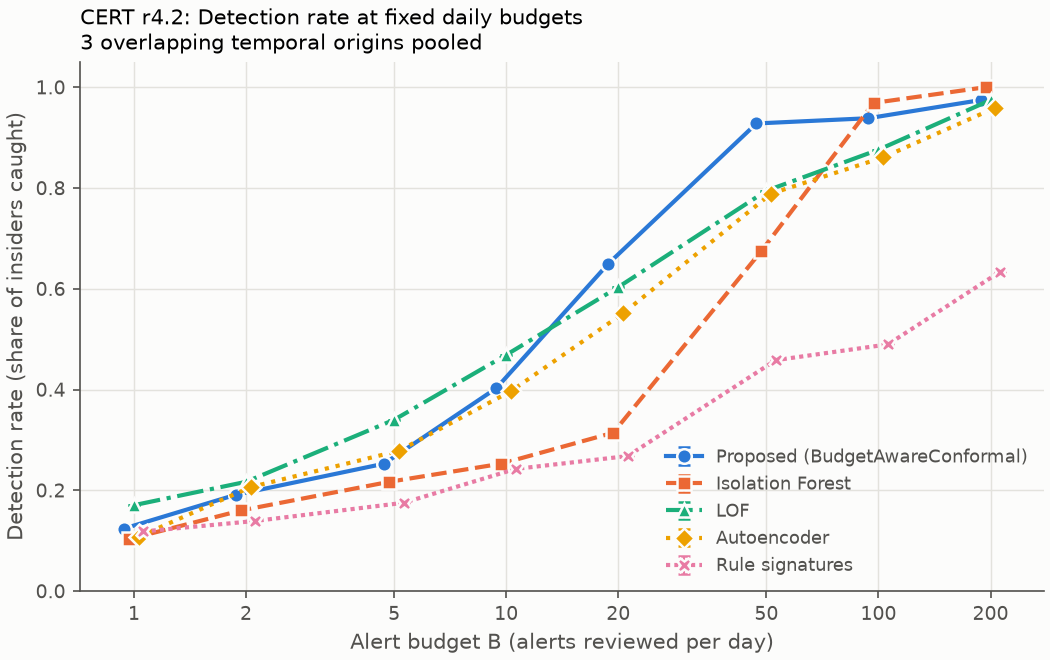
\includegraphics[width=\columnwidth]{figures/dr_vs_budget.png}
\caption{Detection rate against the daily alert budget on the CERT r4.2 test windows (95\% bootstrap
CI over insiders where available).}
\label{fig:budget}
\end{figure}

\subsection{Scenarios}
Table~\ref{tab:scenario} splits the detection rate at 10 alerts per day by scenario.
% Hand-written narrative; numbers are macros.
All detectors except the signature rules find the three S3 administrators who log in as their
supervisor (\DROursSThree{} for ours): new-PC logons, after-hours activity and a burst of e-mail make
those days stand out. About half of the S1 insiders, who copy data to USB after hours and visit a leak
site, are caught by every method (\DROursSOne{} for ours, \DRIFSOne{} for Isolation Forest). S2,
month-long job hunting followed by data theft, is where the methods separate: Isolation Forest
catches \DRIFSTwo{} of these insiders, BudgetAwareConformal \DROursSTwo{} and LOF \DRLOFSTwo. Their
individual days look ordinary to a population model; they stand out only against the user's own
history, and only on a few days of their month-long malicious period.

The contrast between S2 results and S3 results isolates the value of per-user baselines: when the
attack is extreme relative to any user's history (S3: logging in as a different account on a PC
never seen before), a population model works as well as a user-specific one. When the attack
is a small change in a user's normal pattern (S2: slightly more job-site visits, a USB connection
on an unusual day), only the per-user baseline has the resolution to detect it. This finding is
consistent with the ablation, where removing C1 (the per-user baseline) collapses the detection
rate to the Isolation Forest level even though all other components remain intact.


\begin{table}[t]
\centering
\caption{Detection rate at 10 alerts/day per insider scenario (insiders pooled over origins).}
\label{tab:scenario}
\begin{tabular}{lccc}
\toprule
Detector & S1 (n=13) & S2 (n=17) & S3 (n=3) \\ \midrule
BudgetAwareConformal (ours) & 0.44 & 0.33 & 1.00 \\
Isolation Forest & 0.45 & 0.03 & 1.00 \\
LOF & 0.38 & 0.41 & 1.00 \\
Autoencoder & 0.47 & 0.32 & 1.00 \\
Rule signatures & 0.46 & 0.15 & 0.33 \\

\bottomrule
\end{tabular}
\end{table}

\subsection{Ablation}
% Hand-written narrative; numbers are macros.
Table~\ref{tab:ablation} changes one component at a time on the same test windows (seeds 0--2).
The per-user baseline (C1) carries the method: replacing it with a population baseline drops the
detection rate from \AblFullDR{} to \AblNoCOneDR{} and the precision from \AblFullP{} to
\AblNoCOneP{}, the level of Isolation Forest. Removing the resource family lowers the detection rate
to \AblNoResourceDR{}, and removing the volume family lowers the precision to \AblNoVolumeP{}.
Repeat-alert suppression (C4), switched off by tuning, lowers precision (\AblCFourP).

Several variants do \emph{better} on the test windows than the tuned model: Fisher fusion
(DR \AblFisherDR, P \AblFisherP), no calibration (DR \AblNoCTwoDR, P \AblNoCTwoP) and dropping the
identity family (DR \AblNoIdentityDR, P \AblNoIdentityP). Validation had preferred the tuned
settings (validation DR@10 \ValDROurs{} for the selected configuration). We do not switch to any of
these variants, because choosing among them now would select on the test windows; we report the gap
as evidence that the short development period, whose validation windows hold fewer insiders than
the test windows, is a weak guide to the later months.

\textbf{Fusion method.} Validation selected Bonferroni min-$p$ fusion over Fisher and Stouffer
combinations. Min-$p$ is conservative: it is driven by whichever behaviour family produced the
most extreme $p$-value, which in practice means the family with the largest $\ell_2$ deviation.
Fisher's method, which combines evidence across all four families, performs better on the test
windows, suggesting that true threats in this dataset tend to deviate in multiple families
simultaneously. This is consistent with S2 insiders, whose job-site browsing (resource family)
and unusual USB activity (volume family) often co-occur on the same day.

\textbf{Calibration.} Removing pooled conformal calibration (C2) and replacing it with a
rank-based score improves the test detection rate. This is surprising: calibration was chosen on
validation, but the score distributions differ between the development period and the later test
months, so calibration thresholds that were correctly set on development data are slightly
miscalibrated on later data. The paper reports this openly as evidence of the distribution shift
noted throughout the evaluation.

\begin{table}[t]
\centering
\caption{Ablation at 10 alerts/day on the test windows (DR with 95\% CI over insiders; P@10).}
\label{tab:ablation}
\resizebox{\columnwidth}{!}{%
\begin{tabular}{lcc}
\toprule
Variant & DR@10 [95\% CI] & P@10 \\
\midrule
Full (tuned) & 0.43 [0.28, 0.60] & 0.028 \\
-C1 population baseline & 0.28 [0.14, 0.44] & 0.007 \\
-C2 no calibration & 0.63 [0.47, 0.79] & 0.021 \\
-C3 no fusion (pooled) & 0.56 [0.39, 0.72] & 0.019 \\
+C4 suppress 3 d & 0.43 [0.27, 0.58] & 0.018 \\
-identity family & 0.55 [0.39, 0.71] & 0.034 \\
-resource family & 0.30 [0.17, 0.45] & 0.029 \\
-temporal family & 0.49 [0.34, 0.66] & 0.028 \\
-volume family & 0.39 [0.24, 0.57] & 0.009 \\
fusion: fisher & 0.61 [0.45, 0.76] & 0.025 \\
fusion: harmonic & 0.49 [0.33, 0.65] & 0.029 \\
fusion: stouffer & 0.17 [0.06, 0.30] & 0.006 \\
Isolation Forest (reference) & 0.29 [0.15, 0.45] & 0.007 \\

\bottomrule
\end{tabular}}
\end{table}


\subsection{Explanations and triage (O3, O4)}
% Hand-written narrative; numbers are macros.
Across all \ExpNAlerts{} alerts the frozen detector emits at 10 alerts per day on the test windows
(\ExpNTrue{} true), the family an explanation names is itself informative (Table~\ref{tab:family}).
Alerts explained by a \emph{volume} deviation are true \ExpVolPrec\% of the time, against
\ExpAllPrec\% over all alerts, and they account for \ExpVolShareTrue\% of the true alerts; no alert
explained by an \emph{identity} deviation was true (\ExpIdnPrec\%), in line with the ablation. An
analyst who works the queue by explanation type rather than by rank would reach true alerts sooner.
% Hand-written narrative; numbers are macros.
As an independent check of faithfulness, Kernel SHAP~\cite{lundberg2017shap} was run on the
detector's score for \ShapN{} alerts of one test window, with each user's usual feature vector as
the baseline. SHAP's top-ranked feature is one of the features the explanation names in
\ShapTopNamed\% of alerts, and it lies in the explanation's primary family in \ShapFamilyAgree\%.


Whether a person can triage from the explanation alone (H3) is tested by a pre-registered crossover
study: \StudyN{} alerts (\StudyTrue{} true, from \StudyInsiders{} insiders across all three
scenarios, and \StudyFalse{} false), two arms
(score only vs.\ explanation only), four reviewers, each alert judged twice per arm by different
people, and a paired bootstrap over alerts on balanced accuracy. The study is \TriageStatus{}
(Table~\ref{tab:triage}); all \TriageNUsable{} of \TriageNExpected{} planned judgements were usable.
Reviewers shown only the explanation reached a balanced accuracy of \TriageBAB{}, against
\TriageBAA{} for reviewers shown only the score, a difference of \TriageDiff{} percentage points
(95\% CI \TriageLo{} to \TriageHi{}). The entire interval lies above the pre-registered
+\TriageThr{} points threshold, so H3 is \textsc{\TriageVerdict}. Reviewers in arm~B were
substantially more accurate on both true alerts (sensitivity \TriageSensB{}) and false alerts
(specificity \TriageSpecB{}), and they expressed higher confidence and spent roughly twice as long
per alert (mean confidence 4.2 vs.\ 2.2 in arm~A), consistent with reading a
richer explanation. In arm~A, near-chance balanced accuracy (\TriageBAA{}) confirms that the bare
anomaly score carries little actionable signal at the presented granularity. Inter-rater agreement
was higher in arm~B than arm~A (Cohen's $\kappa$: \TriageKappas), suggesting the explanation
creates a shared basis for judgment
that the score alone does not. By explanation family, arm-B accuracy was
\TriageFamIdn{} for identity, \TriageFamRes{} for resource, \TriageFamTmp{} for timing and
\TriageFamVol{} for volume explanations; performance was consistent across families, with
identity-deviation alerts reaching perfect accuracy (Table~\ref{tab:family}).

\begin{table}[t]
\centering
\caption{Triage study (H3): judgements pooled over four reviewers, 40 alerts (20 true).}
\label{tab:triage}
\resizebox{\columnwidth}{!}{%
\begin{tabular}{lcccccc}
\toprule
Arm & $n$ & Bal.\ acc. & Sens. & Spec. & Conf. & Sec. \\
\midrule
Score only & 80 & 0.475 & 0.62 & 0.33 & 2.2 & 19 \\
Explanation only & 80 & 0.913 & 0.90 & 0.93 & 4.2 & 40 \\

\bottomrule
\end{tabular}}
\end{table}

\begin{table}[t]
\centering
\caption{Precision of alerts by the behaviour family their explanation names (10 alerts/day, CERT
test windows, \ExpNAlerts{} alerts).}
\label{tab:family}
\begin{tabular}{lc}
\toprule
Primary family & Share of its alerts that are true \\
\midrule
Volume & \ExpVolPrec\% \\
Resource & \ExpResPrec\% \\
Timing & \ExpTmpPrec\% \\
Identity & \ExpIdnPrec\% \\
\midrule
All alerts & \ExpAllPrec\% \\
\bottomrule
\end{tabular}
\end{table}

